\documentclass[fontsize=12pt, paper=a4, headinclude, twoside=false, parskip=half+, pagesize=auto, numbers=noenddot, open=right, toc=listof, toc=bibliography]{scrreprt}

%\usepackage[inner=4cm,outer=2cm]{geometry}
%\setlength{\oddsidemargin}{15,5pt}
%\setlength{\evensidemargin}{15,5pt}


%parskip:
  % full - Absätze haben großen Abstand
  % half - Absätze haben kleinen Abstand
  % off - Absätze haben Einzug (default)

% Bessere Unterstützung für PDF-Features
\usepackage[breaklinks=true]{hyperref}

%Schönere Schriftart laden
%\usepackage[latin1]{inputenc}
\usepackage[T1]{fontenc} % Ligaturen, richtige Umlaute im PDF
\usepackage[utf8]{inputenc}% UTF8-Kodierung für Umlaute usw
\usepackage[english]{babel} % Deutsche Silbentrennung verwenden
\usepackage{lmodern}
\renewcommand*\familydefault{\sfdefault}  %Zusatz für serifenlose Schrift.

%Zeilenabstand
\usepackage{setspace} % Zeilenabstand
\onehalfspacing % 1,5 Zeilen

% Schriften-Größen
\setkomafont{chapter}{\Huge\rmfamily} % Überschrift der Ebene
\setkomafont{section}{\Large\rmfamily}
\setkomafont{subsection}{\large\rmfamily}
\setkomafont{subsubsection}{\large\rmfamily}
\setkomafont{chapterentry}{\large\rmfamily} % Überschrift der Ebene in Inhaltsverzeichnis
\setkomafont{descriptionlabel}{\bfseries\rmfamily} % für description Umgebungen
\setkomafont{captionlabel}{\small\bfseries}
\setkomafont{caption}{\small}



% Einfachere Verwendung von korrekten Anführungszeichen
\usepackage[german=guillemets]{csquotes}
% oder german=quotes
% oder english=british oder english=american

%Mathematisches
\usepackage{amssymb}
\usepackage{amsmath}
\usepackage{amsthm}

%Quelltext einbinden
\usepackage{algorithm}
\usepackage{algorithmic}

%Abbildungen
\usepackage{graphicx}
\usepackage{caption}
\usepackage{subcaption}
\usepackage[verbose]{wrapfig}
\usepackage{float}
%\restylefloat{figure} %kannst du einen weiteren Positionierungsparameter [H] definieren. der setzt dir das bild an genau die stelle, wo du es haben willst. Ist allerdings auch nicht immer so praktisch.
% wenn du ein \pagebreak einfügst, gibt er dir vor der neuen seite noch alle gleitobjekte aus, die noch anstehen

%Zeichnen mit Tikz
\usepackage{tikz}
\usetikzlibrary{intersections,positioning,shapes.geometric,calc}

% Tabellen
\usepackage{multirow} % Tabellen-Zellen über mehrere Zeilen
\usepackage{multicol} % mehre Spalten auf eine Seite
\usepackage{tabularx} % Für Tabellen mit vorgegeben Größen
\usepackage{longtable} % Tabellen über mehrere Seiten
\usepackage{array}

%Bibliographie
\usepackage[square, comma, numbers, sort&compress, round]{natbib}
\usepackage{bibgerm} % Umlaute in BibTeX

%Umbenennung der vordefinierten definition- und example-Umgebung
\theoremstyle{definition}
\newtheorem{lecture}{Lecture}
\newtheorem{definition}{Definition}
\newtheorem{example}{Example}
\newtheorem{lemma}{Lemma}

% \newtheorem{theorem}{Satz}
% \newtheorem{constructing instructions}{Konstruktionsvorschrift}
% \newtheorem{properties}{Eigenschaften}
%\newtheorem{proposition}{Proposition}
%\newtheorem{korollar}{Corollary}
%\newtheorem{remark}{Remark}
%\newtheorem{consequences}{Consequences}
%\newtheorem{observation}{Observation}
%\newtheorem{conjecture}{Conjecture}
%\newtheorem{recall}{Recall}

\renewcommand{\labelenumi}{\roman{enumi})}

\renewcommand{\labelitemii}{$\bullet$}

\newcommand{\todo}[1]{
      {\colorbox{red}{ TODO: #1 }}
}
\newcommand{\todotext}[1]{
      {\color{red} TODO: #1} \normalfont
}

%bzgl `tocbasic` Warnung
\usepackage{scrhack}
 % Importiere die Einstellungen aus der Präambel
% hier beginnt der eigentliche Inhalt

\author{Lydia Buntrock}
\title{master thesis}
\date{Januar 2018}

% \hfuzz=\maxdimen \tolerance=10000 \hbadness=10000

\begin{document}
  % Titelseite
  \begin{titlepage}
    \pagestyle{empty}
  	
    	\vspace{20mm}
    	\begin{Large}
    	    \textbf{Origins and losses of parasitism}\\
          an analysis of the phylogenetic tree of life with a parsimony-like algorithm\\
    	\end{Large}

  	\clearpage
  \end{titlepage}

%---------------------------------------------------------------------------------------------------
%---------------------------------------------------------------------------------------------------
%--------------------------------------------------------------------------------------------------- 
\chapter*{Abstract}

\tableofcontents
\clearpage

%---------------------------------------------------------------------------------------------------
%---------------------------------------------------------------------------------------------------
%--------------------------------------------------------------------------------------------------- 
\chapter{Introduction}
  \anmerkungstext{Alle Figures richtig beschriften. Generell: Alle Figure captions sollten selbsterklärend sein. Sprich, ich sollte 
    nur die Caption (normalerweise auch unter dem Bild) lesen und nicht den Rest das Papers und dann 
    trotzdem verstehen können, was eigentlich passiert ist und - hilfreich - auch warum das relevant 
    ist. (Bernhard)} \\ \\

  \anmerkung{allgemein zu diesem Kapitel:} \\
  \anmerkung{Eine Einleitung hat etwa 2 Seiten. General problem -> more specific problem (Emanuel)}
  \anmerkungstext{Die Intro ist noch arg knapp =) und ich erkenne die Struktur noch nicht ganz.
    Mein Vorschlag einer Gliederung (jeweils ca. ein Absatz)1) Motivation: \\
      * Was ist das große Ziel? Was soll erreicht werden \\
      * Warum ist das relevant? Was könnte man dann tun? \\
    2) Hintergrund \\
      * Was gab es in dieser Richtung bereits als ganze Ansätze oder wenn nicht, warum nicht? Woran 
        ist es bisher gescheitert  \\
      * welche Grundlagen sind notwendig: \\
      ** open tree of life: Was ist das, warum relevant und überlegen als reine Ansätze? \\
      ** Algorithmen: Was gibt es? Ruhig ausführlicher als hier bereits und vor allem auch nach einer 
        Darstellung am Ende ableiten, was für uns relevant ist. Also beschreiben, wie Methode a, b, c 
        funktionieren und dann abwägen, was daher für Dich am relevantesten ist. \\
    3) Outlook/Structure of this work (Bernhard)} \\

  This paper is about the further development of parsimony algorithms for non-binary trees, applied 
  to the currently largest phylogeny synthesis tree of Open Tree Of Life, with the application to 
  the ancestral state reconstruction of parasitism. \\
  \anmerkung{Der erste Satz muss nochmal überarbeitet werden. Das Ziel / Ergebnis der Arbeit hat sich 
    inzwischen geändert} \\
  \anmerkungstext{Wir haben mehr einen Algorithmus getestet und an unserem spezifischen Problem angewendet, 
    als viel selbst zu entwickeln. Allerdings haben wir den Fitch Algorithmus von binär auf multinär 
    umgeschrieben.} \\
  
  Researchers of the phylogenies have been dealt with the ancenstral state reconstruction in the 
  60s. The first methods were only brute force \todo{Quelle, siehe Fitch: Camin and Sokal 1965}. 
  Next came a set of parsimony algorithms such as: Fitch-parsimony \cite{Fitch1971}, 
  Wagner-parsimony \cite{Swofford1987} ... \todo{weitere?}. \\
  With more and more data, there is now the possibility to use more information to calculate the 
  probabilities of the ancestral states. In addition to the states of the leafs, algorithms could 
  also use branch lengths. The likelihood based algorithms came more in interest. \\
  Our focus came with another 'data extension'. We wanted to work with the biggest phylogenetic tree 
  that exists at this moment, which goes over all observed species. For most \todo{most?} species 
  there is no 
  phylogeny, but only a taxonomic classification. So the biggest 'phylogenetic tree' is a synthesis 
  of phylogenetic trees filled with a taxonomic tree given by Open Tree of Life \cite{Hinchliff2015}.
  This tree is not binary and therefore the developed algorithms are not directly applicable. \\
  \anmerkung{GloBI und OTL in der Einleitung vorstellen. (Emanuel)}
  In this work, we have looked at the algorithms that are generally suited to our data, to develop 
  them further for the not binary case, and finally to compare their usability with our sythesis 
  tree. \\
  We have decided to consider only parsimony algorithms since we have no information on branch 
  lengths and no other additional information like different transition probabilities of our states.

%---------------------------------------------------------------------------------------------------
%---------------------------------------------------------------------------------------------------
%--------------------------------------------------------------------------------------------------- 
\chapter{Methods}
  \anmerkung{Graphischen Workflow hinzufügen, mehr Motivation und genauer. (Bernhard)}
  
  This work consist of two aspects. One is the application of the algorithm to our question the
    other a simulation of this to proof the credibility of our methods. \\
  The resulting procedure is as follows:
  \begin{enumerate}
    \item Get the real tree and real data for the leaf nodes.
    \item Get metadata of these for a realisitc the simulation.
    \item Build and run the simulation.
    \item Evaluation of parameters for the simulation and the real problem.
    \item Run the resulted algorithm on the original data.
    \item Evalute and interprete results. -> Origins etc...
  \end{enumerate}
  
  % Zur Bewertung der gefundenen / entwickelten algorithmen haben wir eine Simulation ausgeführt.

  % Auf der Anderen Seite haben wir unser reales Problem aufgestellt, für die Algorithmen vorbereitet und 
  % diese angewendet.
  
  %---------------------------------------------------------------------------------------------------
  %---------------------------------------------------------------------------------------------------
  \section{Get data}
    %---------------------------------------------------------------------------------------------------
    \subsection{GloBI}
      For tagging our leave nodes, we use the GloBI (Global Biotic Interactions) database. This database 
        consists of entries of the form: species A interacts with B. \\
      We appointed some interactions, where we know from the biological perspective that the species 
      source or target has to be a parasite or a free-living species. These are the following:
      \begin{lstlisting}
        freeliving_source = ["parasiteOf", "pathogenOf"]
        freeliving_target = ["hasParasite", "hasPathogen"]
        parasite_source = ["preysOn", "eats", "flowersVisitedBy", "hasPathogen", "pollinatedBy", "hasParasite", "hostOf"]
        parasite_target = ["preyedUponBy", "parasiteOf", "visitsFlowersOf", "pathogenOf", "hasHost"]
      \end{lstlisting}
      We build two lists: parasites and free-livings, and add the source or targets of an interaction
        to these. \\
      \todo{klar? Oder Beispiel bringen? (Katze isst Maus -> Katze ist Freilebend)} \\
      % For every interaction from these lists, we get one or two species for our parasite or 
      %   free-living lists.
      \todo{ott id hier erwähnen?} \\
      \todo{einige spezies nicht mit einbezogen, da sie keine OTT id haben, hier könnte man noch verbessern (future work)}
      \todo{You can find all interaction types here: https://github.com/jhpoelen/eol-globi-data/blob/master/eol-globi-lib/src/main/java/org/eol/globi/domain/InteractType.java .}
    
    %---------------------------------------------------------------------------------------------------
    \subsection{OTL}
      \todo{Open Tree of Life}

  %---------------------------------------------------------------------------------------------------
  %---------------------------------------------------------------------------------------------------
  \section{Metadata analysis}
    Properties of real Data - Metadata analysis

    There are some Parameters to find out or notice: \\
    \anmerkungstext{hier unterscheiden zwischen einfachen Zahlen (countings / one dimensional) und 
      komplexen variablen (Emanuel)} \\
    \anmerkungstext{arg}{außerdem zu unterscheiden: Biologische Parameter (transition probabilities), 
      fixe Daten und zu berechnende (multifurcation,...) (Emanuel)}
    \begin{itemize}
      \item transition probabilities of tags
      \item multifurcation
      \item nr of parasites to free-living
      \item nr of unknown nodes 
    \end{itemize}
    \anmerkung{multifurcations und unknown leave nodes sind ähnlich beeinflusst (Emanuel)} \\
    \todo{Hier darauf hinweisen, dass wir für multifurcations und unknown data den einfluss auf die 
      Algorithmen testen.}

    %---------------------------------------------------------------------------------------------------
    \subsection{Countings}
      Some simple countings...\\
      nr of parasites, free-living and unknown nodes ... from whole tree, subtrees...
      \begin{center}
        \begin{tabular}{ | l | p{3cm} | }
          \hline
          Name & Number of \\
          \hline \hline
          interactions & 5346414 \\ \hline
          freeliving species & 51337 (distinct) \\ \hline
          parasite species &  47332 (distinct) \\ \hline
          unused possible species & 57352 (source), 809993 (target) \\
          % number of freelivings: 489179
          % number of freelivings: 42657 (distinct)
          % number of parasites: 3353580
          % number of parasites: 44260 (distinct)
          % number of SAME_AS: 86198
          % number of SAME_AS: 16710 (distinct)
          \hline  
        \end{tabular}
      \end{center}

      

    %---------------------------------------------------------------------------------------------------
    \subsection{Multifurcation}
      \anmerkung{Description/Definition of Multifurcation -> to the Intro (Bernhard)} \\
      \anmerkung{Regressionsanalyse (Bernhard)} \\
      \anmerkung{poisson glm: \#children \~ ~ I phylum -> R fitdist p (Emanuel)} \\
      \anmerkung{different parameters for different taxa? (Emanuel)} \\
      One property of the tree is its ridge of multifurcation. For this we collected for every node its
        number of children (degree $-1$), and plottet this in an histogram, how much nodes we have for 
        every degree. Then we tried to find a function which best discribes this behavior. In figure 
        \ref{fig:HistogramsOfMultifurcations} is this plot shown with three functions, which came 
        \todo{close(st)} to this goal: $\frac{1000000000000000}{x^4}$ (magenta), 
        $\frac{300000000000}{x^3}$ (red) and $\frac{80000000}{x^2}$ (black). \\
      \begin{figure}[h]
        \caption{Histogram of multifurcations and fitting functions}
        \centering
        \label{fig:HistogramsOfMultifurcations}
        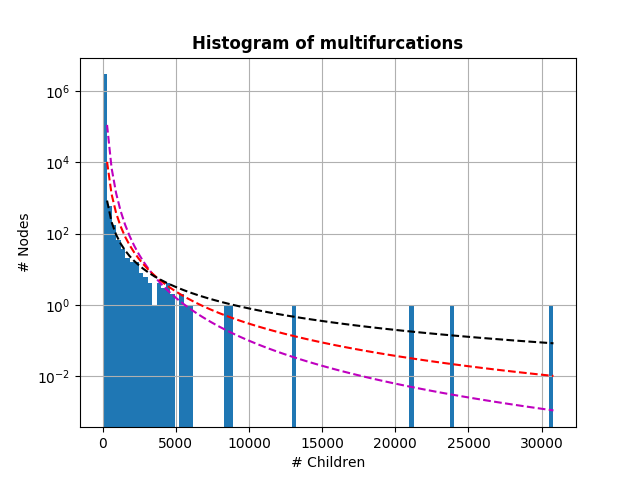
\includegraphics[width=0.7\textwidth]{Figures/HistogramsOfMultifurcations.png}
      \end{figure}
      From the biology we know, that this multifurcation is very clouded. Some parts of the tree are 
        well known and others have not been very interesting for the research so far. So we also wanted 
        to know how the multifurcations behave in some interesting subtrees. \\
      \anmerkung{do we? Is that really universal knowledge or could it be supported by data or a citation? (Bernhard)} \\
      \todo{subtrees... there is some old stuff...} \\
      \todo{other subsections here...} \\

  %---------------------------------------------------------------------------------------------------
  %---------------------------------------------------------------------------------------------------
  \section{Simulation}
    \anmerkung{Motivate the goal of the simulation (Bernhard)}
    \begin{itemize}
      \item build random binary trees, tag these (parameters: parasites vs free-living, 
        beta-distribution)
      \item run fitch-parsimony, wagner-parsimony, our parsimony like algorithm
      \item build not binary tree (poisson distribution?)
      \item run new algorithms
      \item compare trees (distances)
    \end{itemize}

    \begin{enumerate}
      \item build random binary trees
      \item tag tree
      \item multifurcate tree
      \item run maximum parsimony algorithms
      \begin{itemize}
        \item Fitch
        \item Sankoff (Castor package)
        \item my algorithm
      \end{itemize}
      \item Evaluation
    \end{enumerate}

    %---------------------------------------------------------------------------------------------------
    \subsection{random binary tree}
      \anmerkung{Again, motivate first, why this is required and why you choose this solution (Bernhard)} \\
      To get a random binary tree, I used the Phylo package from biopython. They offer a randomized
        function which returns a BaseTree \footnote{
          https://github.com/biopython/biopython/blob/master/Bio/Phylo/BaseTree.py
        }:
      \begin{lstlisting}
        from Bio import Phylo
        Phylo.BaseTree.Tree.randomized(number_leaf nodes)
      \end{lstlisting}
      From the BaseTree class:
      \anmerkung{trivial, does not give real info (Emanuel)}
      \begin{lstlisting}
        def randomized(cls, taxa, branch_length=1.0, 
              branch_stdev=None):
        """Create a randomized bifurcating tree given a list
              of taxa.
          :param taxa: Either an integer specifying the number
              of taxa to create (automatically named taxon#), 
              or an iterable of taxon names, as strings.
          :returns: a tree of the same type as this class.
        """
      \end{lstlisting}
      \todo{Zitat von BaseTree und buildTree.py}

    %---------------------------------------------------------------------------------------------------
    \subsection{tag tree}
      \anmerkung{instead of 'tag tee' simulating stages and transitions between them (Emanuel)} \\
      At this point we want one fully tagged tree, and one less tagged tree which looks like our real 
        data.\\
      Let's say the first specie (the root node) was free-living (start with a parasite without a host 
        makes no sence). For every transition from a node to his child, we take a random number from
        the father distribution. We decided that from the biological perspective a beta distribution
        reflects our transition probabilities best (see Figure 2.1 \todo{ref einfügen}). \\
      \anmerkung{why is that the case and why is that from a biological perspective? (Bernhard)} \\
      \anmerkungstext{I'd rather say that to ensure that the parameter of the binomial distribution is 
        restricted to the [0,1] interval, we model it... (Bernhard)} \\
      For example when our father node was free-living, then we take from the free-living beta
        distribution. Is the number under the threshold for beeing parasite, we get a change and tag
        the current node as parasite. Otherwise we tag it as free-living. \\
      With this procedure we traverse through the tree from the root to every leaf node. A part of
        this code you see here:
      \begin{lstlisting}
        from numpy import random
        if father_tag == 0:
          # freeliving_distribution:
          new_random = random.beta(a=A_FL, b=B_FL)
        else:
          # parasite_distribution:
          new_random = random.beta(a=A_P, b=B_P)
        tag = 0         # -> FL
        if new_random < percentage_parasites:
          tag = 1       # -> P
      \end{lstlisting}
      \begin{figure}
        \caption{60\% Free-living - 40\% Parasites}
        \centering
          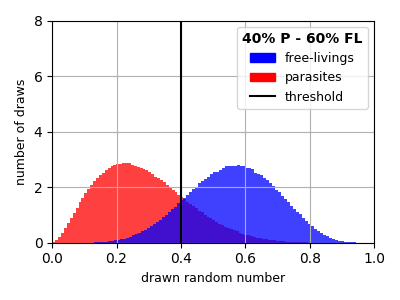
\includegraphics[width=0.5\textwidth]{Figures/40-60.png}
      \end{figure}
      \todo{Bessere Beschriftung, Plot neu erstellen! U.a. mit threshold} \\
      We save each tag with the associated node ID in a nodelist. \\
      \anmerkung{simulationg loss of information (1) states (2) topology/multifurcation (Emanuel)} \\
      The real tree has much less information, we have only information from some current species 
        (leaf nodes) and \todo{and probably negligible internal nodes}. \\
      To simulate our real tree we save for every node an empty placeholde except for some leaf nodes.
      There we save the tags again. The amount of these unknown information is one parameter, which we
      got from our real tree. Or which we can change to \todo{...}
      \todo{Was hiervon gehört ind Methoden, was schon in Implementierung oder ganz woanders hin?}

    %---------------------------------------------------------------------------------------------------
    \subsection{multifurcate tree}
      \anmerkung{simulating loss of information (Emanuel)} \\
      Another parameter is the nature and strength of the multifunction of the tree, since we do not 
        have a binary tree in the real case. After several measurements and analyzes, which we explain 
        in \todo{section/chapter x}, \anmerkung{fit, justification (Emanuel)} we decided to use a $\frac{1}{x}$ distribution, where x is the depth 
        of a node. This means, how deaper we are, how less information we have. \\
      We traverse through the tree and pick a random number between 0 and 1. If random number is smaller 
        as our limit ($\frac{1}{x}$), than we forget the node and hang every child to the father node of 
        the current node. \\
      \anmerkung{poisson process -> fit that distribution, include depth as a predictor, see if significant (Emanuel)}
      \begin{lstlisting}
        from numpy import random
        from utilities import Helpers

        def get_non_binary_tree(subtree, nodelist):
          i = 0
          while i != len(subtree.clades):
            if subtree.clades[i].is_terminal():             # is leaf node?
              i += 1
            else:
              element = Helpers.find_element_in_nodelist(subtree.clades[i].name, nodelist)
              limit = get_limit(element[1])
              new_random = random.uniform()                 # choose if we want to delete ourselve
              if new_random < limit:                        # or new_random < 0.9:
                subtree.clades += subtree.clades[i].clades  # add children
                del subtree.clades[i]                       # delete internal node
              else:                                         # if we don't deleted ourselve go on with children
                get_non_binary_tree(subtree.clades[i], nodelist)  # otherwise the children are in the current clade array
                i += 1
          return

          def get_limit(depth):
            limit = 1 - 1 / ((depth + 3) / 4)
            if limit < 0.1:
              limit = 0.1
            return limit
      \end{lstlisting}
      % # current clades: clade_1 clade_2 ... clade_i-1 clade_i ... clade:_n
      % # add children of clade_i, delete clade_i
      % # new clades:clade_1 clade_2 ... clade_i-1 child_clade_1 ... child_clade_m ... clade:_n
      % # child_clade_1 is new clade i
      Wir lassen das Limit nicht beliebig klein werden, sondern beschränken es auf 0.1.

    %---------------------------------------------------------------------------------------------------
    \subsection{maximum parsimony algorithms}
      \subsubsection{Fitch maximum parsimony}
        Described from [COO98] + others ... - implemented for multifurcating trees

        Fitch algorithm for binary trees:
        \begin{figure}
          \caption{bla}
          \centering
            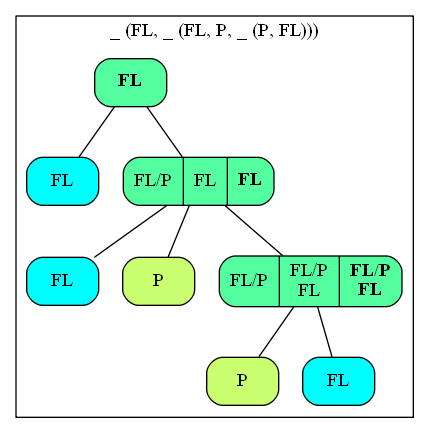
\includegraphics[width=0.5\textwidth]{Figures/Fitch1.png}
        \end{figure}

        Der Baum hat die folgende Struktur: Alle inneren Knoten sind leer. In den Blattknoten befindet 
        sich entweder das Tag FL oder P, oder deren Vereinigung, wenn es sich um einen unknown node handelt.

        Der Fitch Algorithmus ist aufgeteilt in drei Schritte, in welchen man jeweils durch den Baum traversiert.
        Schritt 1 beginnt von de Blättern aus, da sich dort zu Beginn die einzige Information befindet. 
        Für jeden Knoten gilt, wenn seine Kinder schon Information enthalten, dann bilde die Schnittmenge 
        der Tags und schreibe diese als Information in den aktuellen Knoten. Ist die Schnittmenge leer, 
        dann schreibe die Vereinigung aller möglichen Tags in den Knoten. Für alle Kinder, die noch keine 
        Information haben, führe diesen Schritt erst für diese aus.
        Schritt zwei geht von den Kindern der Wurzel bis zu den Vätern der Blätter. Jeder Knoten bekommt 
        einen zweiten Tag, der sich aus der Vereinigung des Tags des Vaterknoten und der Geschwisterknoten
        zusammensetzt. Ist diese leer, bekommt der Knoten wieder die Vereinigung aller Tags, also $\{FL,P\}$ als Tag.

        Hier gibt es einige Möglichkeiten, wie dieser Schritt genau aussieht.
        1. Version: Es wird nur der erste Tag vom Vaterknoten genutzt. Außerdem wird von den 
        Geschwisterknoten zuerst der Schnitt gebildet, und danach vom Ergebnis nochmal mit dem Vaterknoten zusammen.
        (Immer wenn der Schnitt leer ist, ist das Ergebnis die Vereinigung aller Tags, also $\{FL,P\}$. Auch im folgenden...)
        2. Version: Es wird nur der erste Tag vom Vaterknoten genutzt. Er wird zusammen mit den 
        Geschwistertags genommen und direkt ein Schnitt aller Mengen gebildet.
        3. Version: Es werden alle vorherigen Tags vom Vater genutzt und von diesen ein Schnitt gebildet.
        Das selbe gilt für die Geschwistertags. Und dann wird ein dritter Schnitt zwischend en Ergebnissen gebildet.
        4. Version: Es werden alle Tags genutzt und direkt in einem Schnitt zusammengenommen.

        Der Finale Schritt traversiert nochmal über den Baum und Bildet aus den zwei Tags pro Knoten einen finalen
        Tag, indem wieder der Schnitt der beiden Tags das Ergebnis ist.

        Ich habe diese Versionen mit 100 Bäumen mit 10000 Blattknoten und der Verteilung 60\% FL zu 40\% P simuliert.
        Bei 90 \% unbekannten Knoten lag Version 1 zu 89.67 \%, Version 2 zu 89.67 \%, Version 3 zu 
          90.72 \% und Version 4 zu 90.74 \% richtig.

        \begin{figure}
          \caption{bla}
          \centering
            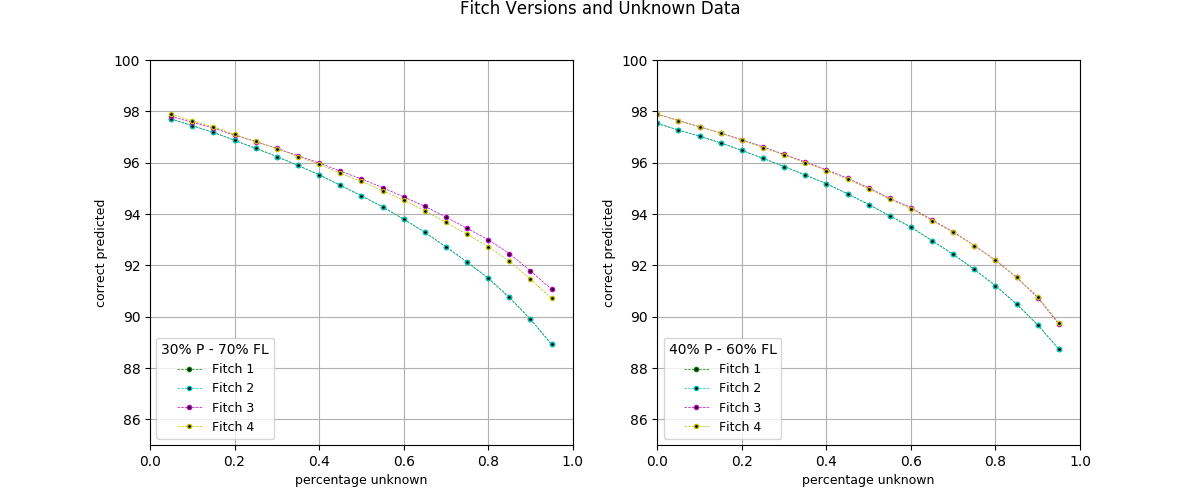
\includegraphics[width=0.6\textwidth]{Figures/simulation_fitch_evaluation.png}
        \end{figure}

        How to extend Fitch for multifunction?:
        \begin{figure}
          \caption{bla}
          \centering
            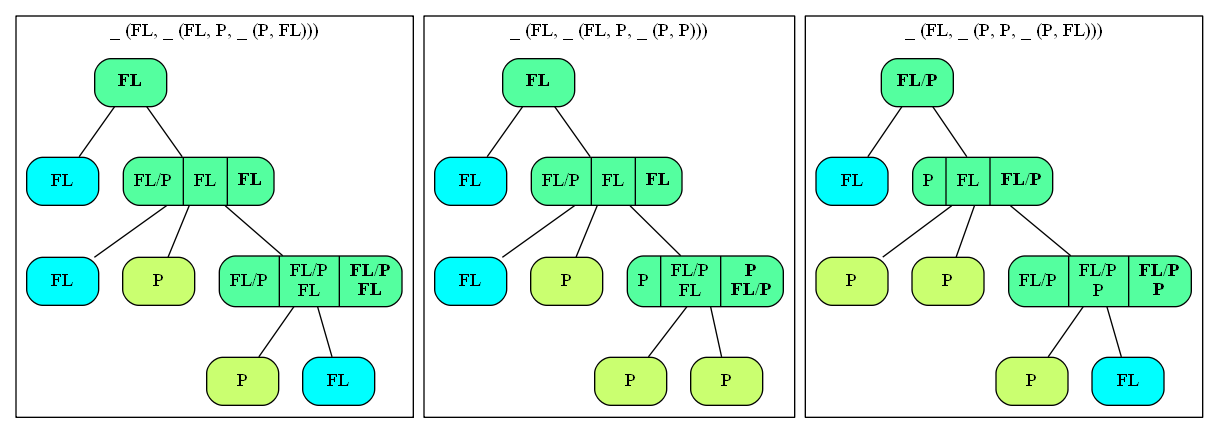
\includegraphics[width=1\textwidth]{Figures/Fitch2.png}
        \end{figure}

      \subsubsection{Sankoff}
        Maximum parsimony algorithm from Sankoff implemented in the R package castor.
      
      \subsubsection{my Algorithm}

  %---------------------------------------------------------------------------------------------------
  %---------------------------------------------------------------------------------------------------
  \section{real data analysis}
    \begin{itemize}
      \item Import tree
      \item Import interactions
      \item run castor algorithm / and others?
      \item interprete results (leave one out)
    \end{itemize}

  %---------------------------------------------------------------------------------------------------
  %---------------------------------------------------------------------------------------------------
  \section{Implementation}

%---------------------------------------------------------------------------------------------------
%---------------------------------------------------------------------------------------------------
%---------------------------------------------------------------------------------------------------
\chapter{Results}

  %---------------------------------------------------------------------------------------------------
  %---------------------------------------------------------------------------------------------------
  \section{Influence of different parameters}

  \begin{figure}
    \caption{Influence of unknown data to prediction}
    \centering
    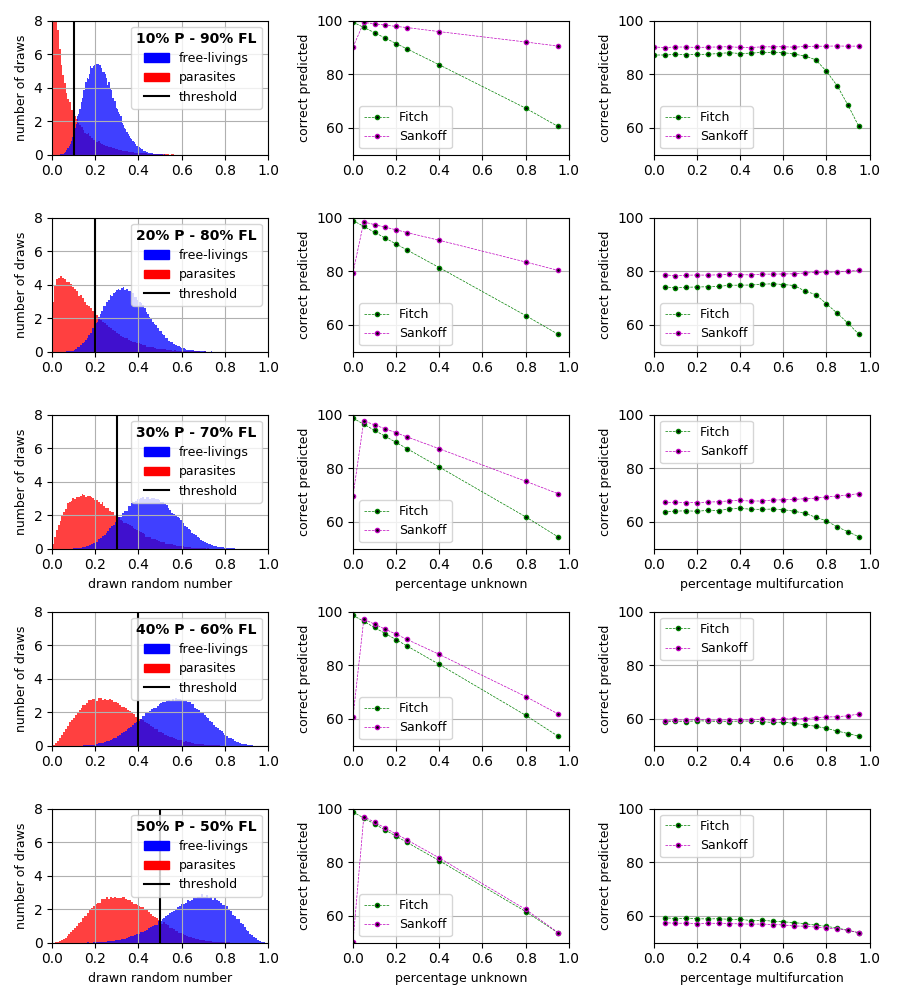
\includegraphics[width=1\textwidth]{Figures/simulation_evaluation_1.png}
  \end{figure}
  

%---------------------------------------------------------------------------------------------------
%---------------------------------------------------------------------------------------------------
%---------------------------------------------------------------------------------------------------
\chapter{Discussion}
  Wie gut ist der randomisiert erstellte Baum? \\
  Wie gut kommt unsere Simulation an die echte Datenlage heran. \\
  Fehlerqoute der Daten an sich? \\
  Wie gut ist unsere Datenlage? 3 mio knoten, 1.8 named species (leaf nodes), 200.000 leaf nodes mit 
  Information. \\
  Simulation von subtrees \\
  Welche Teile des Baumes sind gut, an welchen muss noch viel geforscht werden. \\
  Wieviele Origins haben wir gefunden, was bedeutet diese Zahl? \\
  
  Parameter der Simulation:
  \begin{itemize}
    \item Wie ist die Verteilung der vergessenen internen Knoten? Zum Wurzelknoten hin mehr vergessen?
    \item Wie sehen die übergangswahrscheinlichkeiten aus von P->FL und andersherum?
    \item Verteilung Parasiten zu Freilebend zu keine Information
  \end{itemize}


  Selecting of the 'right'  / best Distribution
  
%---------------------------------------------------------------------------------------------------
%---------------------------------------------------------------------------------------------------
%---------------------------------------------------------------------------------------------------
\bibliography{bibliographie}
\bibliographystyle{alphadin}


\end{document}
